%\usepackage{listings}
\section{A function prediction method}
\subsection*{Prologue}
As we mentioned in the introduction our main goal was to develop
a classification algorithm for the PLC problem which can be used for the
purpose of protein function prediction in a partially annotated PPI
network.

What it means is we are going to take an input a strongly connected
graph where the vertices represent protein types and the edges represent
observed interaction between them. The some of the proteins are
annotated with a label that specifies their function. The rest are
unannotated.

The prediction algorithm outputs a suggested label for each unlabeled protein.
Our paradigm is that protein is that proteins of the
same label should form, approximately, a community in the sense of
graph community structure which we discussed in the earlier sections.
Since the algorithm is using propagation methods which are closely
related to the community structure of the graph, if the paradigm doesn't
hold then the prediction sohould be no better than a coin toss.

It is understood that proteins that interact more likely than not
share the same function~\cite{schwikowski2000network}. It's a weaker
property than our paradigm because it doesn't speak about communities,
only about adjacent proteins.

The diffusion matrix provides us with ranking such that for for every
vertex $i$ we can weigh the other vertices by 'importance' to that
vertice (namely it's the $i$ row of the diffusion matrix). We use that
information to predict the label of the protein. We assume that members
of the same label of the protein will have cumulatively the most
'influence' on it. We also assume that the distribution of labeled and
unlabeled is the same across the network so by removing them from
consideration, still the proteins that share the same label with the
protein we test will have the most cumulative influence on it.

We tested and compared 5 different methods, 3 were diffusion based and 2
were neighbor based which we used mainly as the reference point.

The source code for all the algorithms and the test can be found at
the project's git repository~\cite{project_git}.

\subsection*{The Algorithm}

We tried 5 different prediction methods:

\begin{itemize}
\item{Method 1} Determines the group affiliation of an unknown node
by the group that has the maximal volume based on the propagation
distribution from the unknown node. This meas: we calculate the
stationary distribution with restart to the unknown node. Among the
known nodes, we calculate the weighted sums of each of the 4 groups
according to that distribution. The group with largest volume (see
pseudo code for the decision function below) is the affiliation we
assign to the unknown node.


\item{Method 2} This method works like method 1, except that we first order the
unknown nodes according to their pageRank. We go over the
nodes in this order and assign group affiliation according to method 1, but then
we also update the list of the known nodes to include that node. So this node is
going to be included in the function prediction of the lower ranked nodes.

The rational here was that the RWR as we have seen has the property
that heat flows from the low ranks to the high ranks. So maybe we
should pick a low ranked vertex and see where it flows to.
If we start from a hot central vertex.

\item{Method 3} We assign an unknown node to the group that has plurality among
its neighbors with known group affiliation. So this method is fast and
probably the simplest. This method is essentially the 'prediction
function' from \cite{schwikowski2000network}.

\item{Method 4} Same as method 3, but again we go in the order of pagRanks and
we update the list of known nodes on the fly, like method 2.

\item{Method 5} Here we take each group of the known nodes and propagate from
it. So for example we calculate the stationary distribution when we restart in
the known nodes that belong to group 'DNA Replication', and then for the next
group and so forth. For each unknown node, we assign it to the group that
propagates the highest probability to it.

While in method 1 and 2 we start random walking from an unknown node and see
what is the probability that we land at a certain group, In Method 5 we start
walking randomly from one of the members of a group and check what is the
probability that we visit a certain unknown node.

This method is an order of magnitude faster than method 1 and 2 because we only
need to calculate the stationary distributions 4 times (pageRank and for each
group). However we suspect it will perform with less accuracy.
The reason for that is that method 5 takes into account nodes that are far and not well connected to the
unknown node whose function we try to predict.
The function groups, in particular the yellow (meiosis) and green (stress) are not
well clustered and spread all over the network but we can see that
some subsets of these labels form clusters.

\end{itemize}

\begin{minipage}{\linewidth}
\begin{lstlisting}[mathescape=true, 
    caption = {method 2, decision funciton}, label={code:decision_function}]
# vertices are enumerated 1 to n. labels are enumerated 1 to m.
# input v: vertex of unknown label, to be predicted
# input F: the diffusion matrix (so F is column-normalized)
# input labeledSubset: list of boolean vectors. so
#    if labeledSubset[l] = (1, 0, ...),
#    then vertex 1 has label l and vertex 2 doesn't.

def decisionFunction(v, F, labeledSubset):
  # get p, the influence vector of v, which is column v of F:
  let $p$ = $F \cdot e_v$
  let labeledSums = [sum(p[x]) for x in labeledSubset]
  return argmax(labeledSums)
\end{lstlisting}
\end{minipage}

\begin{minipage}{\linewidth}
\begin{lstlisting}[mathescape=true, 
    caption = {method 2, main funciton}, label={code:method2}]
# vertices are enumerated 1 to n. labels are enumerated 1 to m.
# Input G: a strongly connected graph
# input labeledSubset: list of boolean vectors. so 
#    if labeledSubset[l] = (1, 0, ...),
#    then vertex 1 has label l and vertex 2 doesn't.

def predictionMethod2(G, labeledSubset):
  # calculate the diffusion matrix
  let F = diffusionMatrix(G)
  # calculate the pageRank order
  let pr = $F \cdot \bar{1}/n$
  let unknowOrderedList = [v : v is unlabeled].sort_up_by(pr)
  for v in unknowOrderedList:
    predLabel <- decisionFunction(v,F,labeledSubset)
    # set v's labels to predLabel
    # it will participate in the subsequent predictions
    labeledSubset[predLabel][v] <- 1
  return labeledSubset
\end{lstlisting}
%this is listing \ref{code:decision_function}.
\end{minipage}

\subsection*{Experimental Protocol}
We first constructed a \textbf{fully} labeled subnetwork of the
yeast interactome by choosing arbitrarily 4 labels, the only
constrain was that each labeled subset be sufficiently large (approximately
100 or more nodes).
We then removed from the network all nodes that didn't have one of
those 4 labels: 'DNA replication' (blue), 'Golgi' (red), 'Meiosis'
(yellow), and 'Stress response' (green). We also removed nodes that
had more than one of these 4 labels (of which there were only a
handful). The resulting subnetwork is shown in figure
\ref{fig:yeast_subgraph_4groups}. 
We then selected the greatest connected component of that network,
and this was our experimental graph.
It contains around 500 vertices.

In the first set of tests, we tested the accuracy of each of the 5
methods. We randomly selected 50\% of the nodes and
assigned them to the known group, that is, they were the labeled
subset. The rest were the unlabeled. We ran each of the 5 methods on
this partially labeled networked and validated its accuracy by
comparing its prediction with the fully labeled network. We repeated
these tests twice, on 2 different randomly selected labeled subsets.
The results are in table~\ref{table:results_5_prediction_methods}

We then chose method 2 which had the highest accuracy for further
tests. We tested it with different parameters, repeating each
settings 50 times with 50 different sets of known labels. The
parameters we tested were the restart probability ($\alpha$) and
what we called the \textbf{labeled coverage}, which is the portion
of the nodes that start with a known label.

We have conducted another test of method 2, with parameters $\alpha
= 0.31$, and label coverage of $0.35$. This time we calculated the
sensitivity, specificity, accuracy and precision (PPV) for each
label as well as the total.

\begin{figure}[!htb]
\begin{framed}
\centering
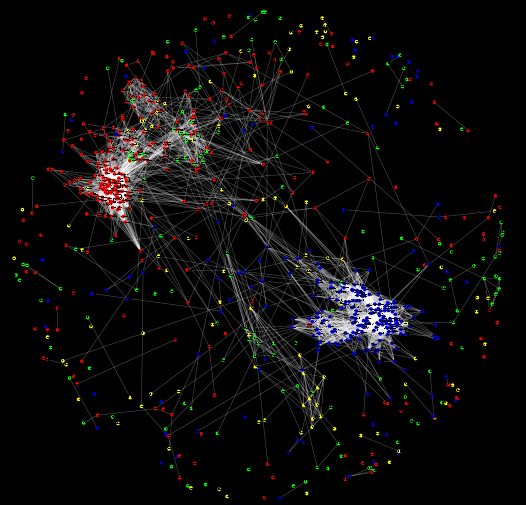
\includegraphics[width=\textwidth]{figures/yeastsubgraph_4_groups_colorcode.png}
\caption{Subgraph of the yeast interactome showing nodes of 4 groups: 'DNA
replication' (blue), 'Golgi' (red), 'Meiosis' (yellow), 'Stress response'
(green)}
\label{fig:yeast_subgraph_4groups}
\end{framed}
\end{figure}

\subsection*{Results}

Table~\ref{table:results_5_prediction_methods} shows the results of
the experimentally measured accuracy for each of the 5 method on 2
50\% labeled networks (the networks are the same, the labeled
vertices were randomly selected). 

\begin{table}[!htb]
\caption{Prediction Accuracy of the 4 Methods in 2 different random
trials. Each trial with a different seed, which result in different randomly
selected known/unknown nodes.} 
\begin{center}
\begin{tabular}{ | l | c | c | c | c | c | }
\hline
Seed / Method & 1 & 2 & 3 & 4 & 5\\
\hline
42 & 0.795 & 0.854 & 0.765 &
0.791 & 0.701\\
6382020 & 0.774 & 0.832 & 0.751 & 0.751 & 0.755\\
\hline
\end{tabular}
\label{table:results_5_prediction_methods}
\end{center}
\end{table}

We picked method 2 which was the best performer for further tests.
Figure~\ref{fig:largest_connected_comp}
shows the network and the hits and misses of the prediction
algorithm method 2.

\begin{figure}[!htb]
\begin{framed}
\centering
\begin{subfigure}[b]{\textwidth}
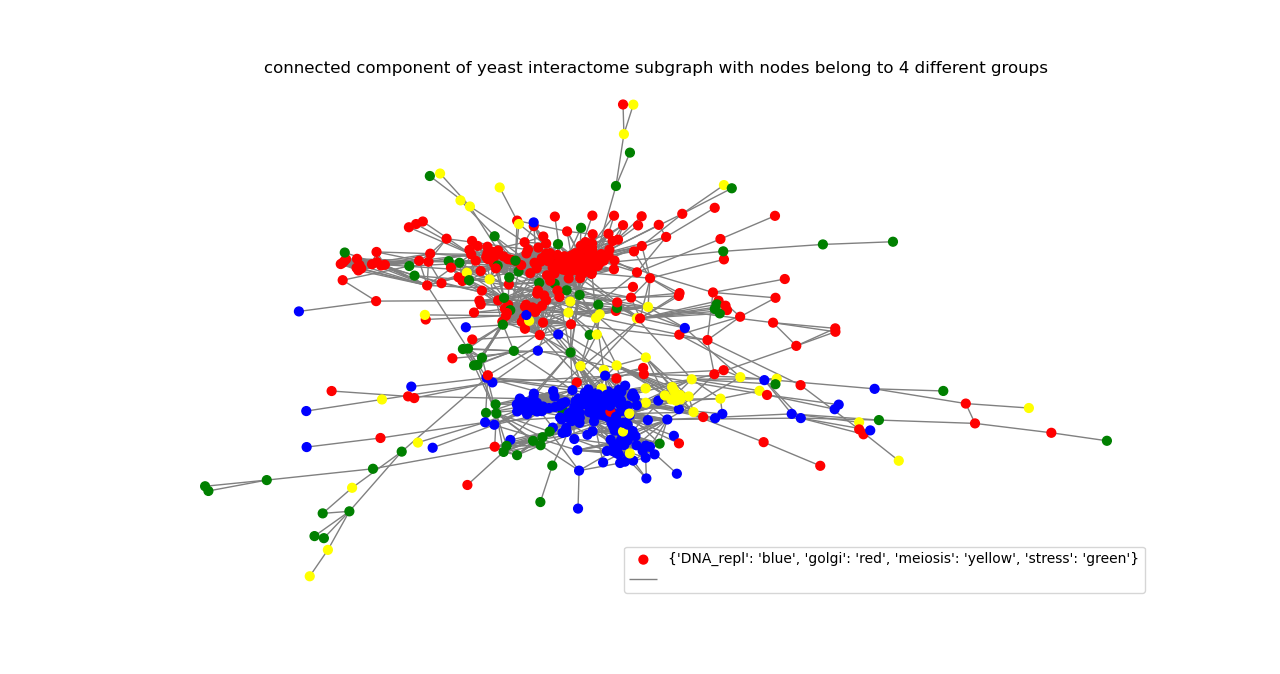
\includegraphics[width=\textwidth]{figures/connected component of yeast interactome subgraph with nodes belong to 4 different groups.png}
\caption{The largest connected component which was selected for the function
prediction experiment. Here the Correct group affiliation of all nodes is color
coded.}
\end{subfigure}
\begin{subfigure}[b]{\textwidth}
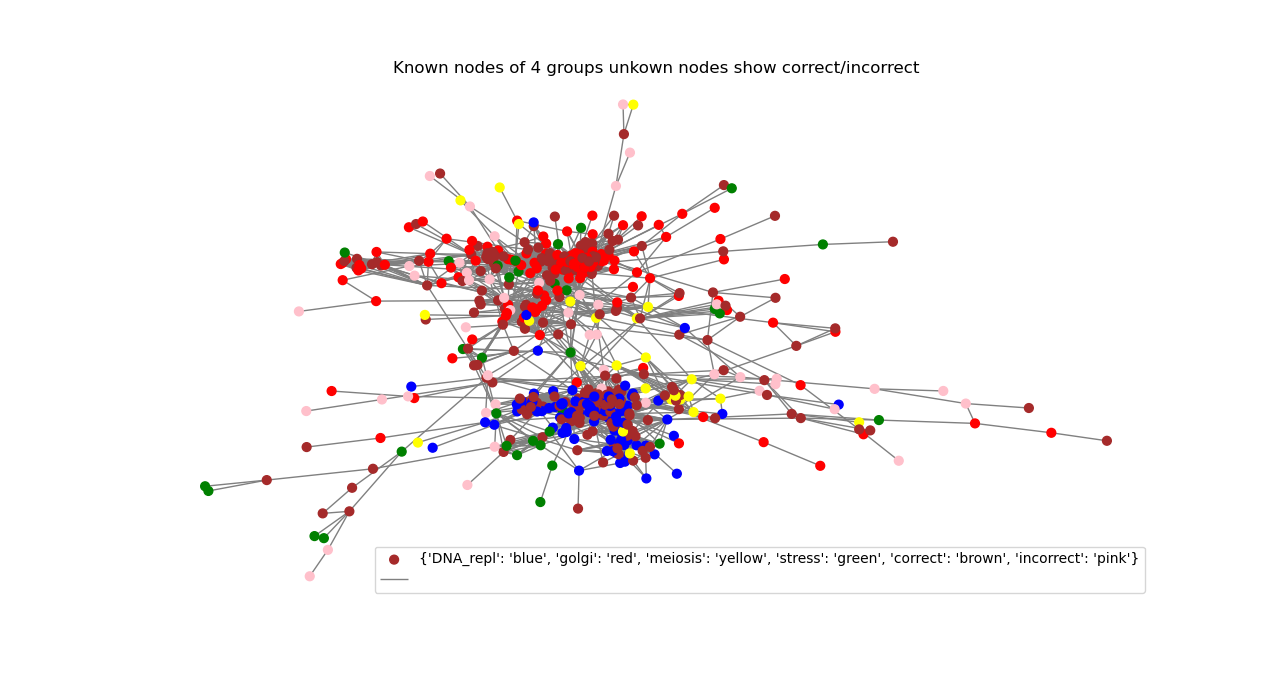
\includegraphics[width=\textwidth]{figures/method2_true_false_clustering_on_4_groups_with_ordering_and_update.png}
\caption{The result of predictiob method 2, which was the best perfomer. 
The known groups are color coded by RGBY. The unkown nodes are color
coded: brown:correct prediction, pink:incorrect.}
\label{fig:my_prediction}
\end{subfigure}
\caption{The test network}
\label{fig:largest_connected_comp}
\end{framed}
\end{figure}

Upon further testing we conducted with method 2,
the best mean result (for coverage of 0.5), was $0.8926$ mean accuracy.
It was obtained with a
restart probability of $0.31$. Restart parameters $\alpha \in [0.2-0.3]5$, lets
call it mid-lower range, produce the best results, while with higher
alphas accuracy falls towards $0.5$ which is of course the accuracy of
just randomly guessing. 

Accuracy was about 0.8 when we start with only 10\% labeled and it
gradually increases with increased labeled proportions (0.85 accuracy at
0.3 label coverage). We plotted the relationship between accuracy and
the parameters in figure \ref{fig:alpha_fracs}.

\begin{minipage}{\linewidth}
We have tested method 2 for accuracy, precision, specificity and
sensitivity, with parameters $\alpha = 0.31$, and label coverage of
$0.35$. The values were calculated for each label as well as the
total. The results are the following:

\begin{lstlisting}[basicstyle=\footnotesize, label=tab:sens]
      Label      P     TP    FP        N       TN    FN Sens Spec  Acc  PPV
0     golgi    165    149    25      209      184    16 0.90 0.88 0.89 0.86
1  DNA_repl    133    129    22      241      219     4 0.97 0.91 0.93 0.85
2   meiosis     30     17     4      344      340    13 0.57 0.99 0.95 0.81
3    stress     46     25     3      328      325    21 0.54 0.99 0.94 0.89
4     Total 374.00 320.00 54.00 1,122.00 1,068.00 54.00 0.86 0.95 0.93 0.86
\end{lstlisting}
\label{tab:senspec}

We can see that the problem lies with the two small and spread out
groups, 'meiosis' and 'stress'. It is hard to predict that an
unlabeled vertex belong to these groups 

\end{minipage}

\begin{figure}[!htb]
\begin{framed}
\centering
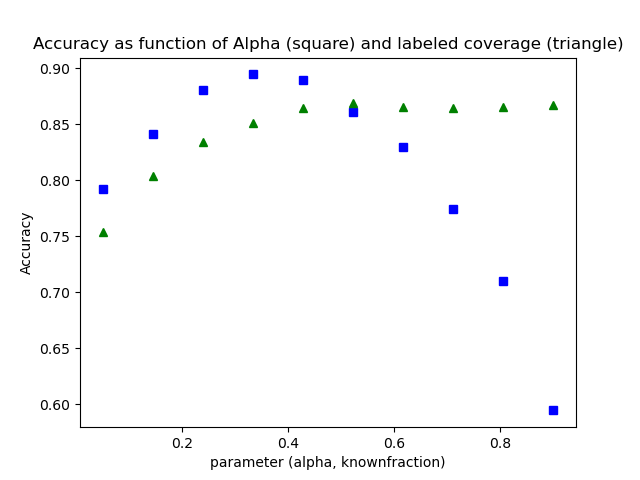
\includegraphics[width=\textwidth]{figures/alpha_fraq_graph.png}
\caption{The accuracy as function of the resart parameter alpha,
with fixed label coverage of 0.5, and of the label coverage with
fixed alpha=0.2}
\label{fig:alpha_fracs}
\end{framed}
\end{figure}

\subsection*{Remarks and Conclusions}

If we look at figure \ref{fig:largest_connected_comp} which shows the connected
component that we worked with, the red and blue are pretty nicely clustered. The
greens and specially the yellows are sort of spread all over the network and
not nicely clustered. We don't know if this is a good example of a real world
scenario in the context of PPI networks.

When we look at figure \ref{fig:my_prediction} it seems that most of the
incorrect predictions are on nodes that seem 'peripheral' and  are not well
connected to known nodes. Another source of mistakes seems to bee green nodes
that are too close to the red cluster.

Method 2 shows somewhat higher accuracy over the other methods but on the flip
side it is an $O(n^2)$ method when optimized methods are used whereas methods
3,4,5 are $O(n)$.

We suspect (but it requires testing) that the accuracy of methods 3
and 4 would decrease more rapidly with decreasing labeled coverage
than it did with method 2. The reason is that methods 3 and 4 become
completely arbitrary on a vertex which has no labeled neighbors.
Method 1,2 rank all the vertices on a graph so they may have a
better chance of finding the right label. 



%Section 4 gave us a strong indication about the usefulness of the
%diffusion matrix as as a type of quasi-distance with which we
%measure closeness or 'influence' between nodes in the network.
%Our working paradigm is that connected nodes are more likely to have
%the same functional class than not, a fact which has been shown to
%be true by \textcite{schwikowski2000network}.
%
%In this section we are going to apply the accumulated knowledge of the
%previous sections and devise some simple function prediction algorithms for PPI
%networks. We to try several methods which use propagation as well as
%methods which just use direct neighbors for the predictions.
%
%The network is going to be composed of around 500 vertices (proteins) which are
%divided into 4 different function groups. We are going to randomly choose half
%the proteins and mark them as unknown and try to predict their function based
%on the remaining known proteins. Then we can verify the results with the
%actual annotations.

%\subsection{Tools and Source Data}
%
%We sourced our data from \textcite{cytoscape}, an open source
%java software for network analysis and visualisation. 
%The software as one of its built in examples a
%fully annotated yeast interactome. This is a PPI network of
%thousands of proteins and it contains among many other types of
%edge and node annotations information about protein function and
%location in the 'MCs name' field.
%
%We preferred to work within the familiar Python 3 programming
%language and its rich world of extension libraries and packages.
%Therefore we exported the yeast interactome into a graphml format
%which was later imported into our network analysis tool of choice,
%\textcite{networkx}. This is a python based open sourced network analysis 
%package which integrates extremely well with other essential Python
%packages. Networkx is neither as versatile nor as powerful as Cytoscape and
%especially rudimentary in its visualisation functionality, but it
%runs smoothly and is easy to work with, unlike Cytoscape.
%We used the \textcite{numpy} package for vector, matrix and other
%types mathematical
%calculations, and \textcite{pandas} for some database operations. 
%
%\subsection{Methodology}
%As mentioned, we 
%used the annotated yeast interactome which is a pure PPI network that comes
%prepackaged with the
%software tool 'Cytoscape'. The nodes represent yeast proteins and the edges
%represent protein-protein interactions.
%
%This network comes with functional annotations in the 'MCs name' field.
%We selected nodes in the network whose annotations contain
%\textbf{exactly} one of the following keywords:  'DNA Replication' (blue
%group), 'Golgi' (red), 'Meiosis' (yellow), and 'Stress response'
%(green). All other nodes are removed from the network.  The result is
%shown in figure \ref{fig:yeast_subgraph_4groups}.
%
%The resulting subnetwork is not a connected graph, which is the type
%of input data that we wanted to run our test algorithm on. Therefore
%we selected the biggest connected component of that subnetwork, and
%that is the graph on which we tested and compared various prediction
%algorithms.
%
%
%For the first set of comparative tests of different prediction
%methods 
%we set a random seed (a process which we repeat 2 times for 2 different trials).
%Then we selected randomly 50\% of the nodes and marked them as 'unknown'. The other
%50\% are 'known'. We would then try to determine the group affiliation of the
%unknown nodes based on the group affiliations of the known nodes.

%We tried 5 different prediction methods:
%
%\begin{itemize}
%\item{Method 1} Determines the group affiliation of an unknown node by the group
%that has the maximal volume based on the propagation distribution from the
%unknown node. This meas: we calculate the stationary distribution with restart
%to the unknown node. Among the known nodes, we calculate the weighted sums of
%each of the 4 groups according to that distribution. The group with largest
%volume is the affiliation we assign to the unknown node.
%
%\item{Method 2} This method works like method 1, except that we first order the
%unknown nodes (decreasing order) according to their pageRank. We go over the
%nodes in this order and assign group affiliation according to method 1, but then
%we also update the list of the known nodes to include that node. So this node is
%going to be included in the function prediction of the lower ranked nodes.
%
%The rational here is that the higher ranked nodes are probably going to be
%predicted with high accuracy and therefore be helpful in prediction of lower
%ranked nodes. 
%
%It is probably better to device some simple rule to decide whether it is worth
%to include a node in the prediction of the rest of the nodes. For example, based
%on how many unknown neighbors in has vs known neighbors. But we tried to keep
%things simple at this stage.
%
%\item{Method 3} We assign an unknown node to the group that has plurality among
%its neighbors with known group affiliation. So this method is fast and
%probably the simplest.
%
%\item{Method 4} Same as method 3, but again we go in the order of pagRanks and
%we update the list of known nodes on the fly, like method 2.
%
%\item{Method 5} Here we take each group of the known nodes and propagate from
%it. So for example we calculate the stationary distribution when we restart in
%the known nodes that belong to group 'DNA Replication', and then for the next
%group and so forth. For each unknown node, we assign it to the group that
%propagates the highest probability to it.
%
%While in method 1 and 2 we start random walking from an unknown node and see
%what is the probability that we land at a certain group, In Method 5 we start
%walking randomly from one of the members of a group and check what is the
%probability that we visit a certain unknown node.
%
%This method is an order of magnitude faster than method 1 and 2 because we only
%need to calculate the stationary distributions 4 time (pageRank and for each
%group). However we suspect it will perform with less accuracy.
%The reason for that is that method 5 takes into account nodes that are far and not well connected to the
%unknown node whose function we try to predict.
%The function groups, in particular the yellow (meiosis) and green (stress) are not
%well clustered and spread all over the network but we can see that
%some subsets of these labels form clusters.
%
%\end{itemize}


%\subsection{Results}

%\begin{table}[!htb]
%\caption{Prediction Accuracy of the 4 Methods in 2 different random
%trials. Each trial with a different seed, which result in different randomly
%selected known/unknown nodes.} 
%\begin{center}
%\begin{tabular}{ | l | c | c | c | c | c | }
%\hline
%Seed / Method & 1 & 2 & 3 & 4 & 5\\
%\hline
%42 & 0.795 & 0.854 & 0.765 &
%0.791 & 0.701\\
%6382020 & 0.774 & 0.832 & 0.751 & 0.751 & 0.755\\
%\hline
%\end{tabular}
%\label{table:results_5_prediction_methods}
%\end{center}
%\end{table}

%We decided to further experiment with method 2.
%We tested it with different parameters, repeating each settings 50 times
%with 50 different sets of known labels. The parameters we tested were
%the restart probability ($\alpha$) and what we called the labeled
%coverage, which is the portion of the nodes that start with a known
%label.
%The best mean result (for coverage of 0.5), was $0.8926$ mean accuracy.
%It was obtained with a
%restart probability of $0.31$. Restart parameters $\alpha \in [0.2-0.3]5$, lets
%call it mid-lower range, produce the best results, while with higher
%alphas accuracy falls towards $0.5$ which is of course the accuracy of
%just randomly guessing. 
%
%Accuracy was about 0.8 when we start with only 10\% labeled and it
%gradually increases with increased labeled proportions (0.85 accuracy at
%0.3 label coverage). We plotted the relationship between accuracy and
%the parameters in figure \ref{fig:alpha_fracs}.
%
%\begin{figure}
%\begin{framed}
%\centering
%\begin{subfigure}[b]{\textwidth}
%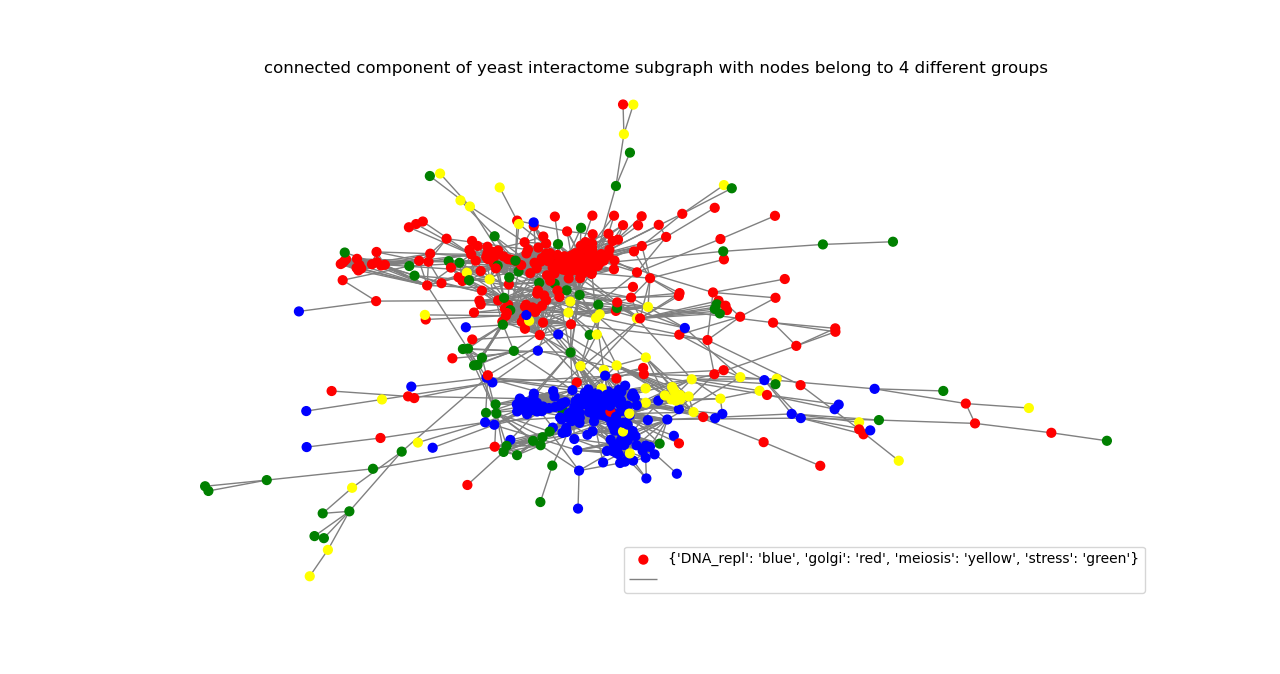
\includegraphics[width=\textwidth]{figures/connected component of yeast interactome subgraph with nodes belong to 4 different groups.png}
%\caption{The largest connected component which was selected for the function
%prediction experiment. Here the Correct group affiliation of all nodes is color
%coded.}
%\label{fig:largest_connected_comp}
%\end{subfigure}
%\begin{subfigure}[b]{\textwidth}
%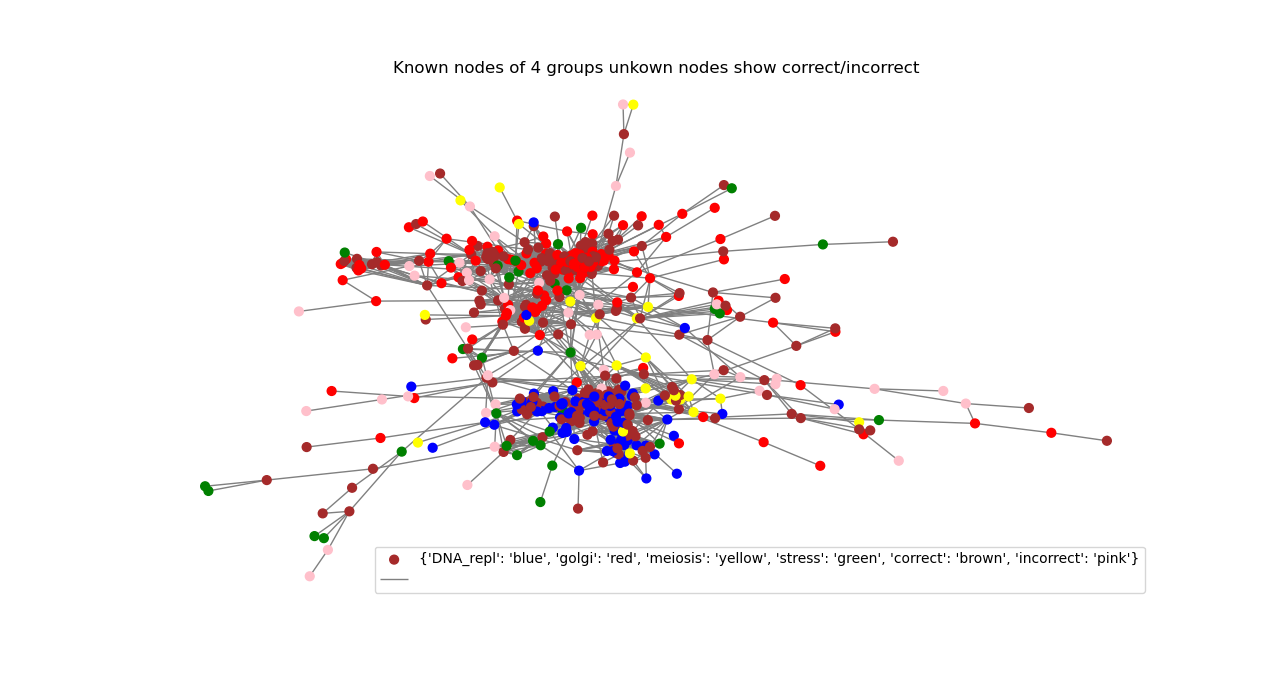
\includegraphics[width=\textwidth]{figures/method2_true_false_clustering_on_4_groups_with_ordering_and_update.png}
%\caption{The result of predictiob method 2, which was the best perfomer. 
%The known groups are color coded by RGBY. The unkown nodes are color
%coded: brown:correct prediction, pink:incorrect.}
%\label{fig:my_prediction}
%\end{subfigure}
%\end{framed}
%\end{figure}
%
%We have conducted another test of method 2, with parameters $\alpha =
%0.31$, and label coverage of $0.35$.
%This time we calculated the sensitivity, specificity, accuracy and
%precision (PPV) 
%for each label as well as the total.
%The results are the following:
%\begin{lstlisting}[basicstyle=\footnotesize]
%      Label      P     TP    FP        N       TN    FN Sens Spec  Acc  PPV
%0     golgi    165    149    25      209      184    16 0.90 0.88 0.89 0.86
%1  DNA_repl    133    129    22      241      219     4 0.97 0.91 0.93 0.85
%2   meiosis     30     17     4      344      340    13 0.57 0.99 0.95 0.81
%3    stress     46     25     3      328      325    21 0.54 0.99 0.94 0.89
%4     Total 374.00 320.00 54.00 1,122.00 1,068.00 54.00 0.86 0.95 0.93 0.86
%\end{lstlisting}
%\label{tab:senspec}
%
%We can see that the problem lies with the two small and spread out groups,
%'meiosis' and 'stress'. It is hard to predict that an unlabeled vertex belong to these groups 
%
%\begin{figure}
%\begin{framed}
%\centering
%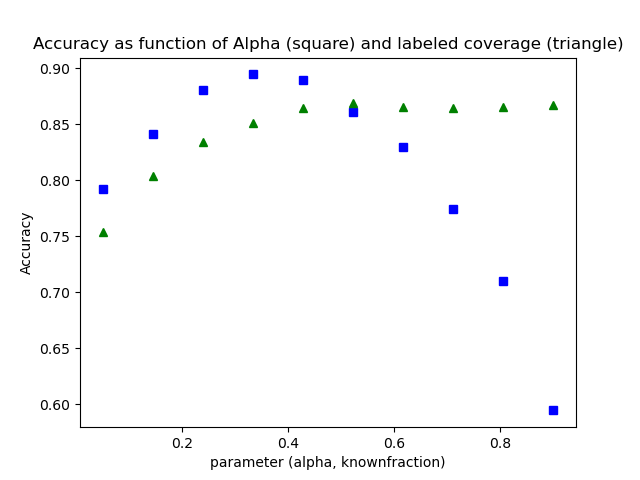
\includegraphics[width=\textwidth]{figures/alpha_fraq_graph.png}
%\caption{The accuracy as function of the resart parameter alpha,
%with fixed label coverage of 0.5, and of the label coverage with
%fixed alpha=0.2}
%\label{fig:alpha_fracs}
%\end{framed}
%\end{figure}

%\subsection{Discussion}
%If we look at figure \ref{fig:largest_connected_comp} which shows the connected
%component that we worked with, the red and blue are pretty nicely clustered. The
%greens and specially the yellows are sort of spread all over the network and
%not nicely clustered. I don't know if this is a good example of a real world
%scenario.
%
%When we look at figure \ref{fig:my_prediction} it seems that most of the
%incorrect predictions are on nodes that seem 'peripheral' and  are not well
%connected to known nodes. Another source of mistakes seems to bee green nodes
%that are too close to the red cluster.
%
%Method 2 shows somewhat higher accuracy over the other methods but on the flip
%side it is an $O(n^2)$ method when optimized methods are used whereas methods
%3,4,5 are $O(n)$.
